

\chapter{Integral Image Algorithm}
 The \textit{integral image algorithm}, also known as \textit{summed area table} is a two-dimensional table generated from an input image. Integral image is a very popular and important algorithm in computer vision and computer graphics applications. Especially in real-time computer vision, it is usually used to accelerate calculating the sum of a rectangular area. 
 
  The aim of the IIA is to calculate the sum of values in a rectangular subset of a grid. In particular, the final value of a point inside a grid can be written as:
  
  \begin{equation} \label{eq:IIA eq}
  I(x,y)=\sum\limits_{x'=1}^{x}\sum\limits_{y'=1}^{y}  i(x',y')
  \end{equation}
   
   As shown in the figure \ref{fig:IIA}, the value of the dark blue rectangle can be calculated as the sum of all the light blue rectangles.
   
 
  	\begin{figure}[h]
  		\centering
  	 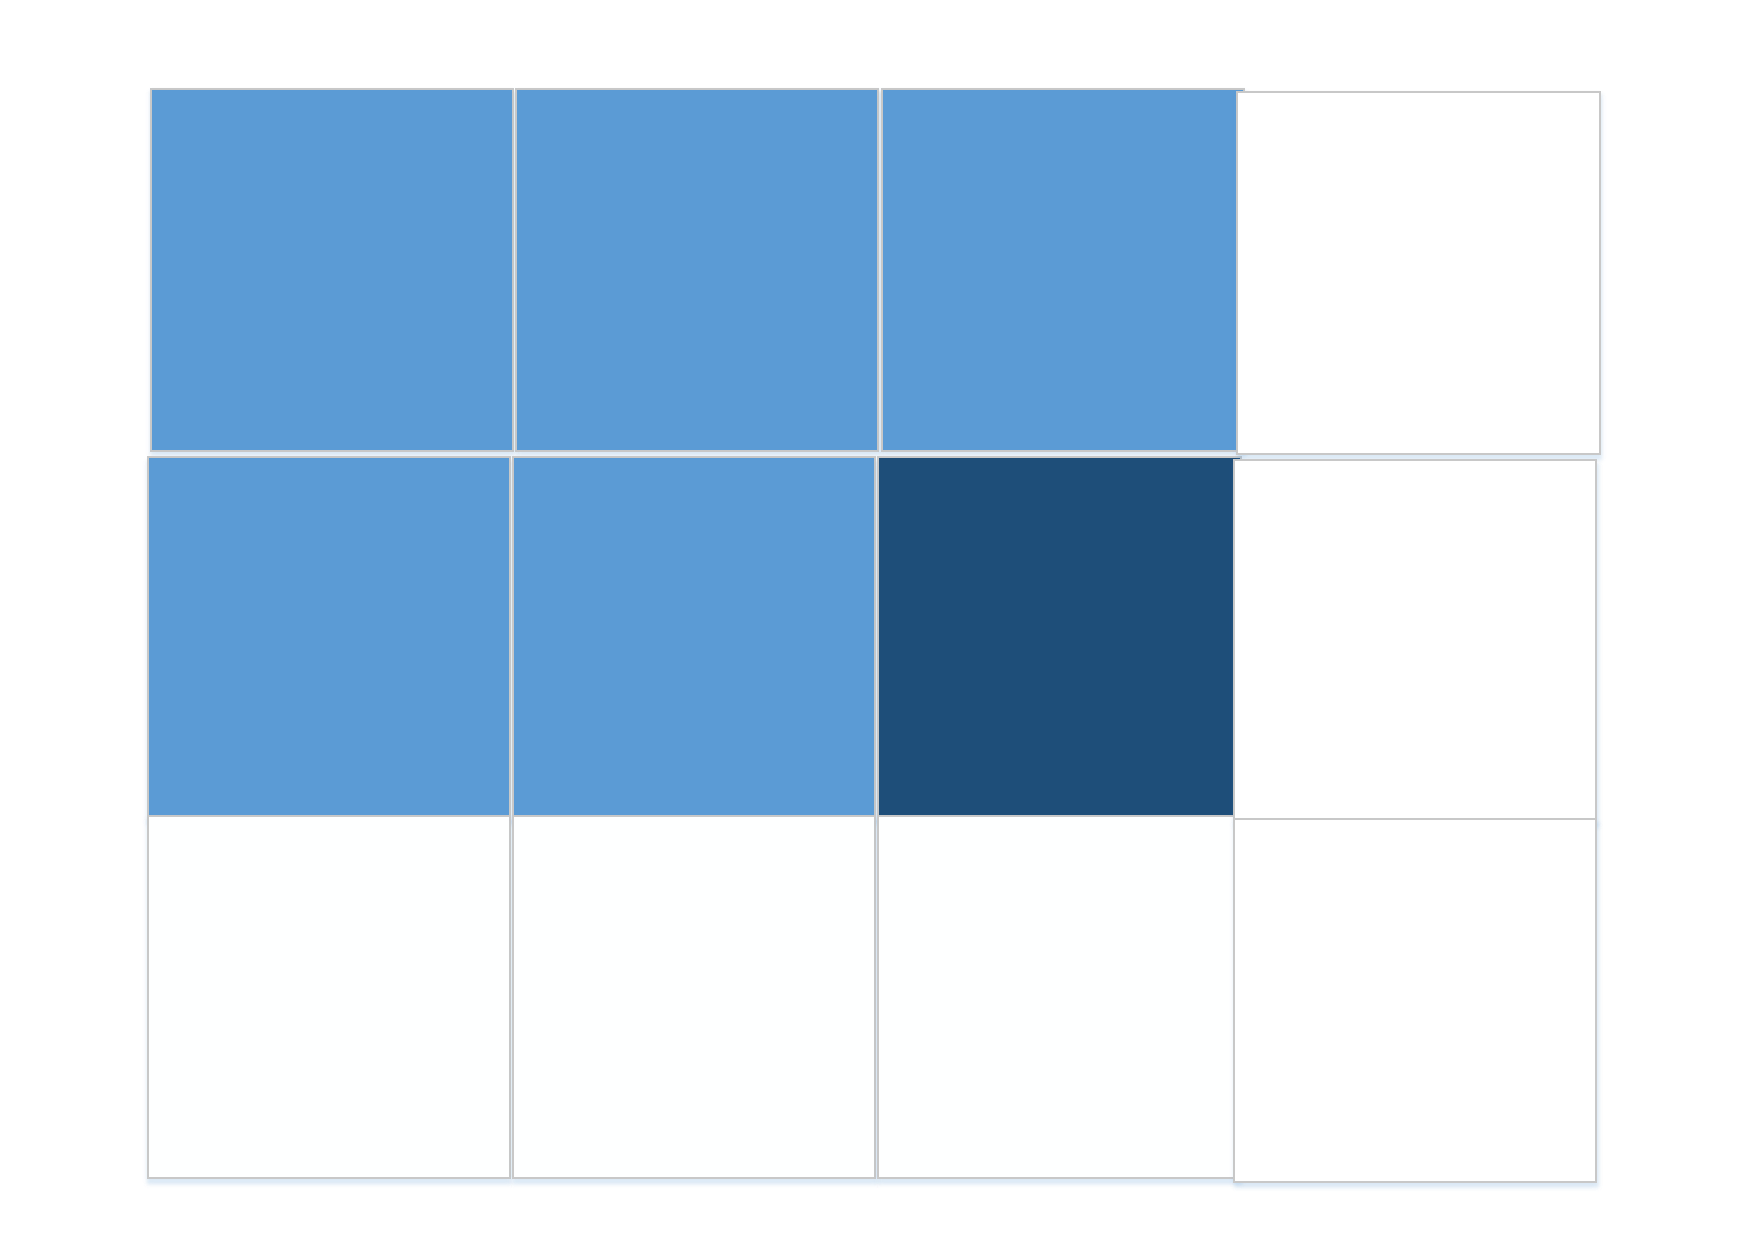
\includegraphics[scale=0.25]{imm/iia/Disegno1}  
   \caption{SAT of a single cell}
   \label{fig:IIA}
\end{figure}
  
 \section{Method used}
 I decided to use the approach ASAP (as soon as possible), so in this implementation we try to maximize the parallelism.
 To better explain, we first look to the Integral Image of a 1D array.
 At each step \textit{i} we have the array  partitioned in array of size $ 2^{i} $, and each of them has its own integral image values.\\
 In the next step \textit{i+1}, we pair two consecutive array of size $ 2^{i} $, (thus having an array of $ 2^{i+1} $) and do the Integral image. \\Since we have already computed the partial integral image, for the new one, the elements from \textit{1} to $ 2^{i} $ has the correct values, while for the elements from $ 2^{i} $ to $ 2^{i+1} $ we need to sum the value stored in position $2^{i} $.
 Figure \ref{fig:iia0} represents this method, while figure \ref{fig:iia1} shows an example of an 8-array.
 
   	\begin{figure}[h]
   		\centering
   		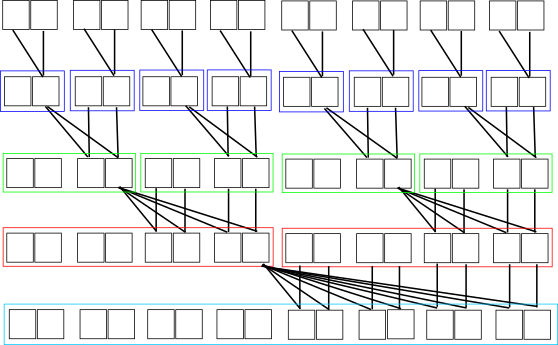
\includegraphics[width=\textwidth]{imm/iia/iia00.png}  
   		\caption{Schematic of the SAT of a 1D array}
   		\label{fig:iia0}
   	\end{figure}
   	
   	  	\begin{figure}[h]
   	  		\centering
   	  		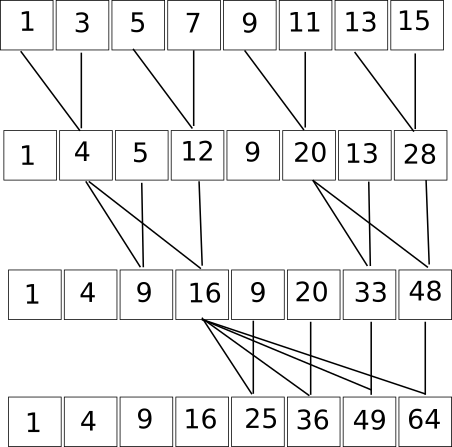
\includegraphics[width=\textwidth]{imm/iia/iia1.png}  
   	  		\caption{SAT of a 1D array with some values}
   	  		\label{fig:iia1}
   	  	\end{figure}
  When we want to handle the integral image of a 2D array, we can compute the same method both vertically and horizontally. 	  	
   	  	\clearpage
  \section{Hardware Implementation} \label{hiiia}
  The algorithm has been properly implemented for an ASIC architecture that privileges the throughput (i.e. computes as fast as possible).
   The pseudocode is the following:
   \begin{enumerate}
   	
   	\item Divide the NxN matrix into small 2x2 matrices and compute the corresponding summed area table (SAT).
   	This step is shown in figures \ref{fig:IIA1} and \ref{fig:IIA1a}
   	
   	  \begin{figure}[h]
   	  	\centering
   	  	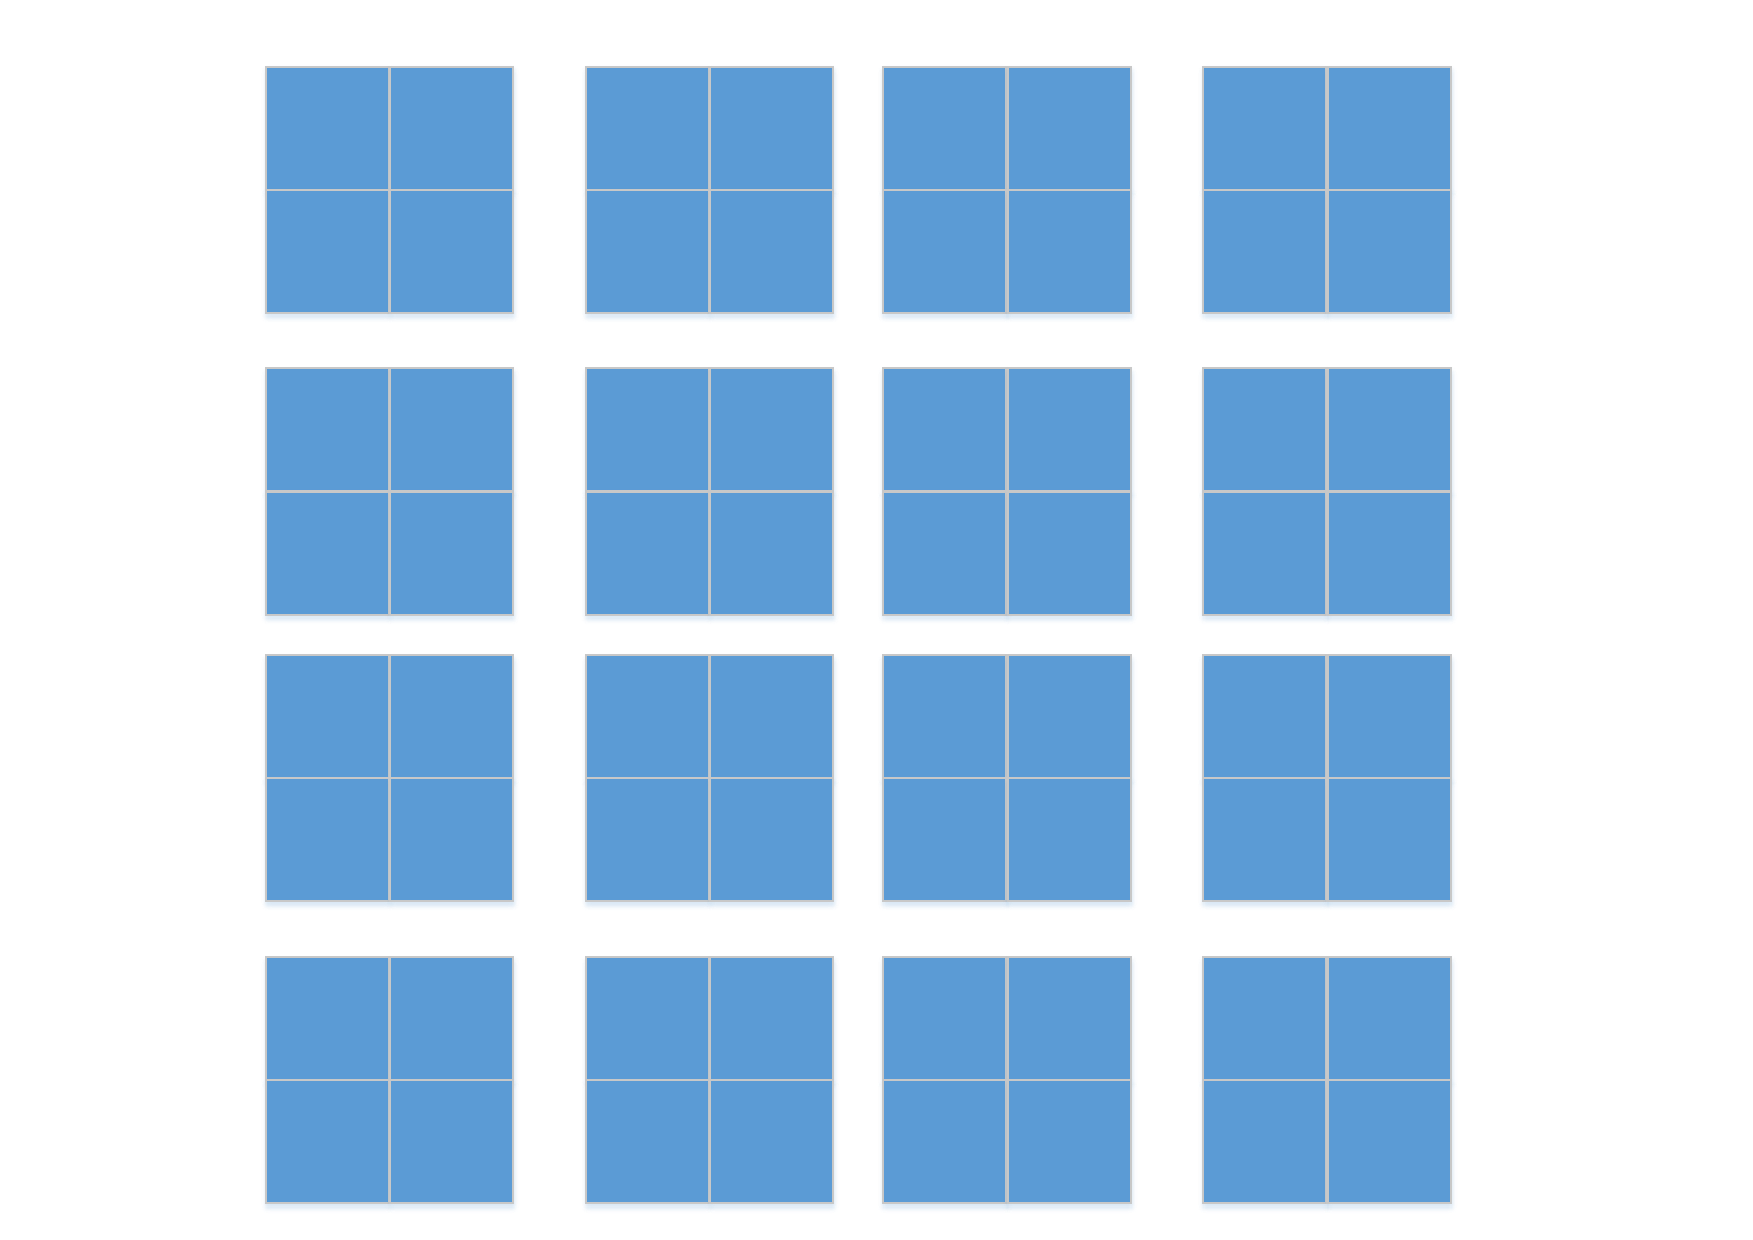
\includegraphics[scale=0.45]{imm/iia/iia_step1}  
   	  	\caption{ Subdivision in 2x2 matrices} 
   	  	\label{fig:IIA1}
   	  \end{figure}
   	
   \begin{figure}[h]
   	\centering
   	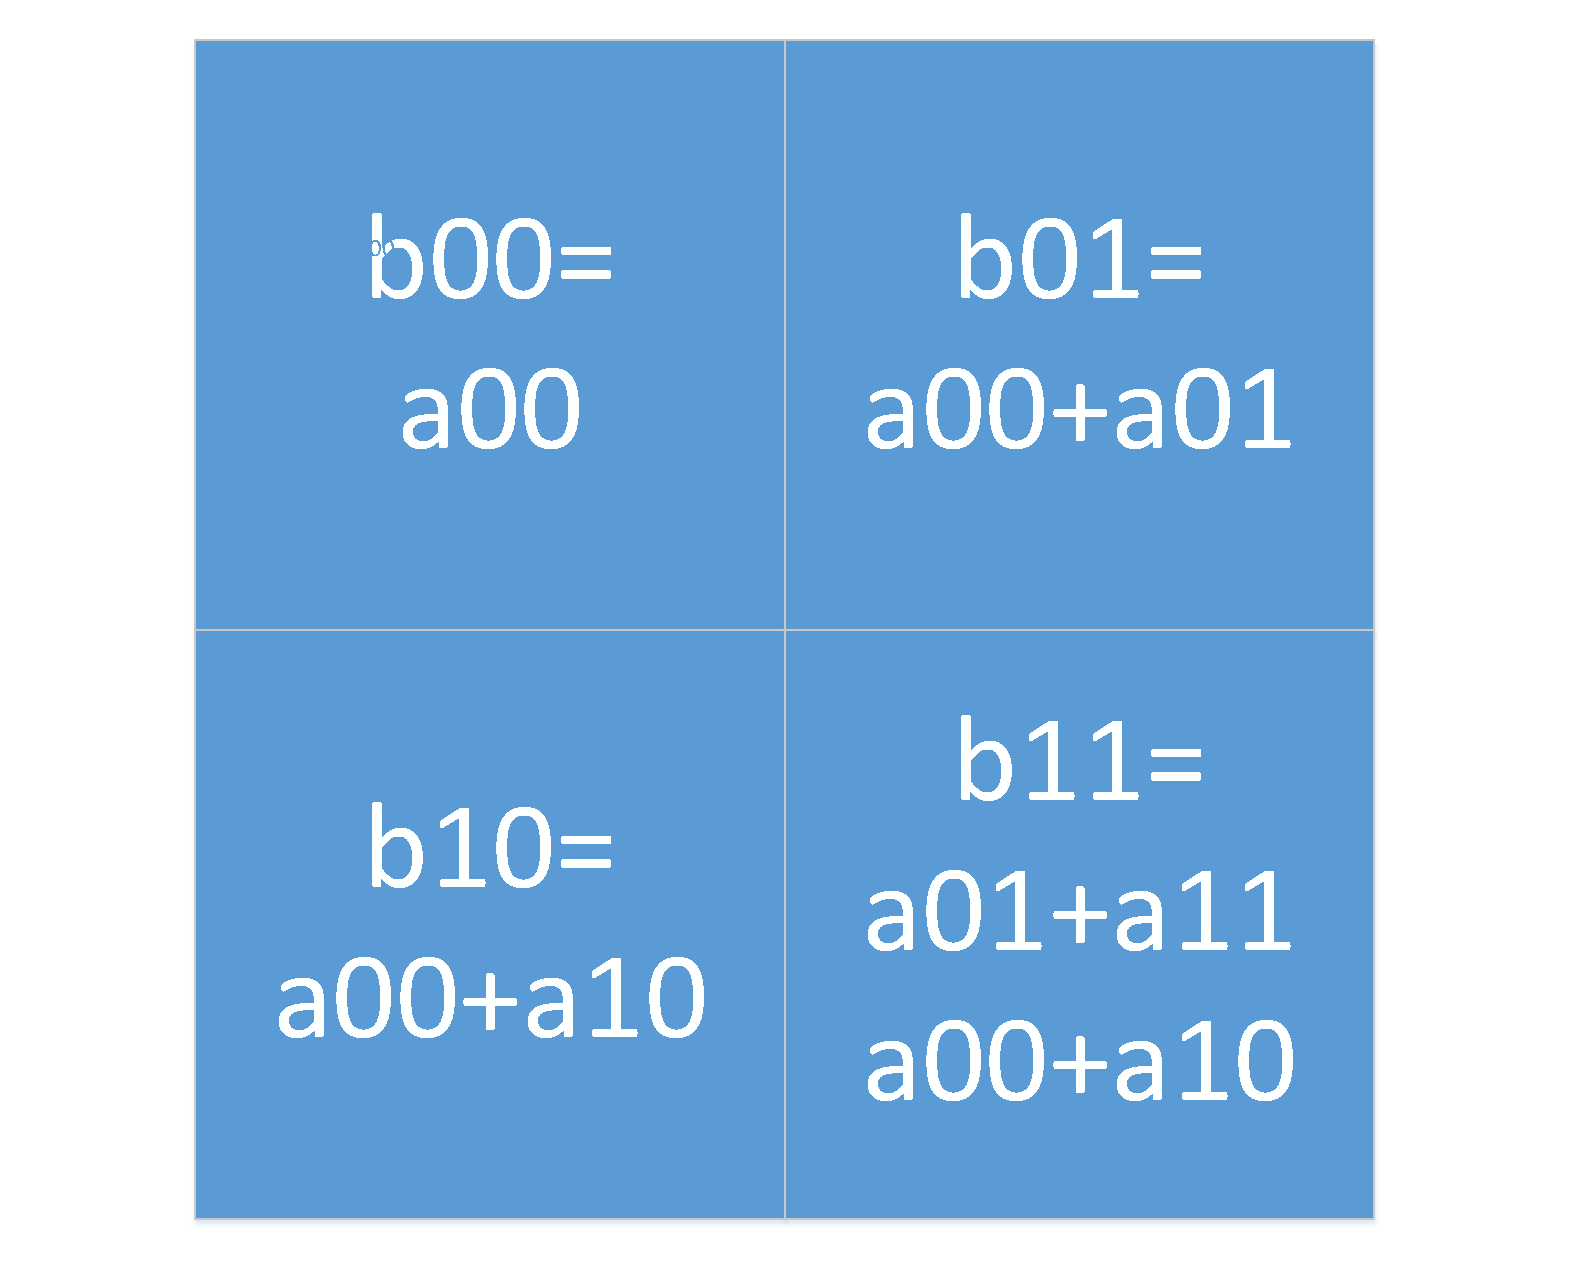
\includegraphics[scale=0.25]{imm/iia/iia_step1a}  
   	\caption{SAT of a 2x2 matrix} 
   	\label{fig:IIA1a}
   \end{figure}
   
 
   
   	\item Group all the above matrices into 4 matrices and evaluate the corresponding SATs.
   	The computation will be faster because we have some partial SATs.
   	When we sum vertically, we just sum to all the lower half cells with the corresponding cell of the last row of the upper half matrix. This is done because the last row of the upper half contains the partial SAT of the small matrices computed in the previous step.
   	Figure \ref{fig:IIA2aa} shows that after this operation the left half side of this 4x4 matrix has its SAT computed.
   	Similarly we sum horizontally: as shown in figure \ref{fig:IIA2b} we add to all cells of the right side the corresponding cell of the last column of the left half matrix. Now all cells of this 4x4 matrix has the SAT computed
   	
   	   \begin{figure}[h]
   	 \centering
   	   	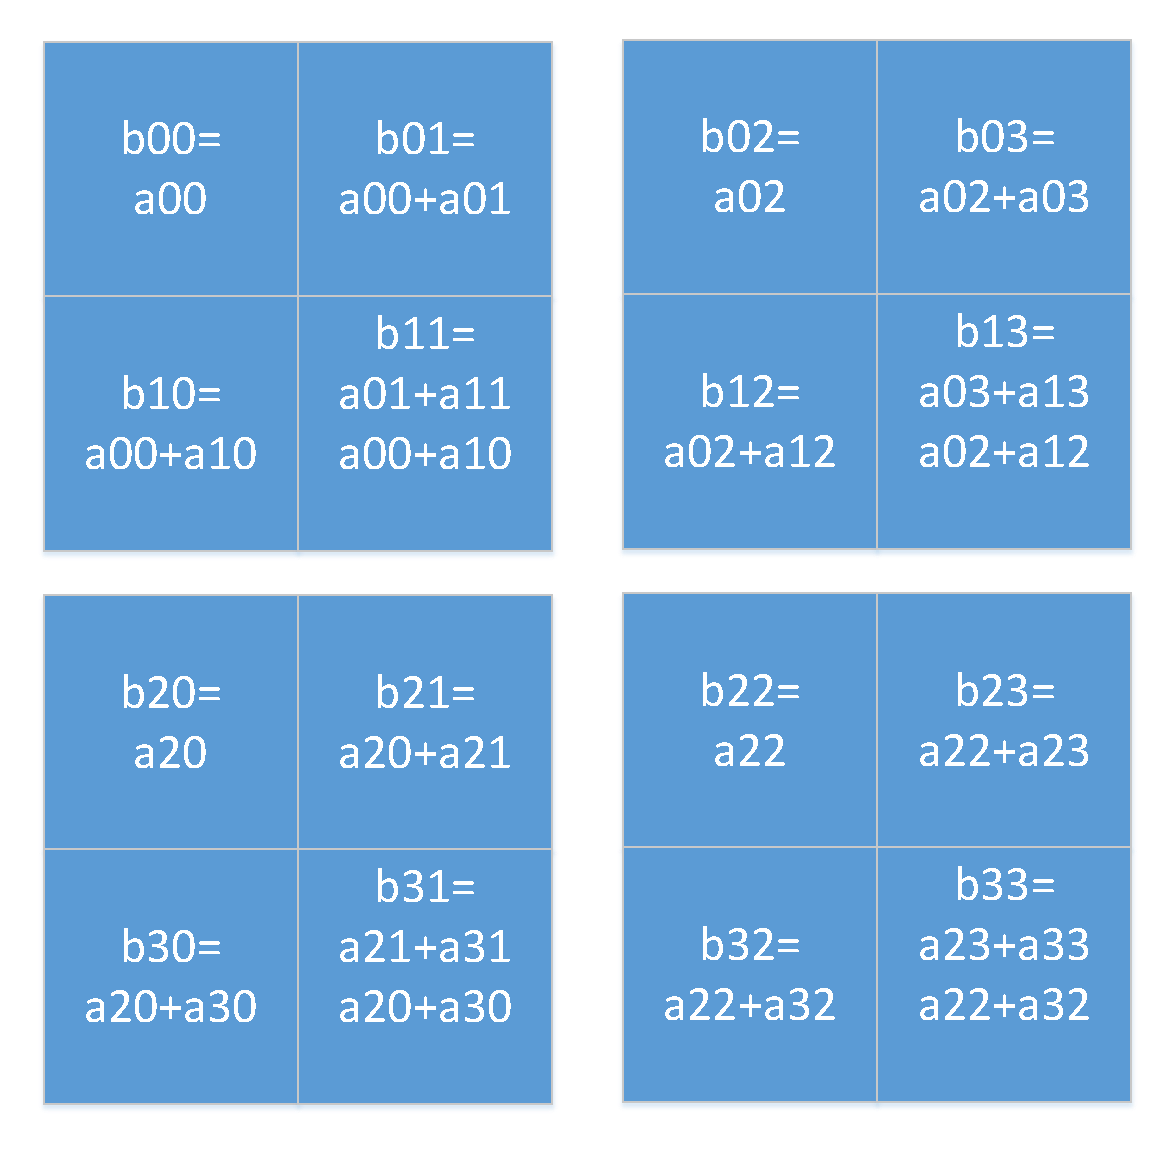
\includegraphics[scale=0.40]{imm/iia/iia_step2a}  
   	   	\caption{Step 2-Initial state of a 4x4 matrix} 
   	   	\label{fig:IIA2a}
   	   \end{figure}
   	   
   	   \begin{figure}[h]
   	   \centering	
   	   	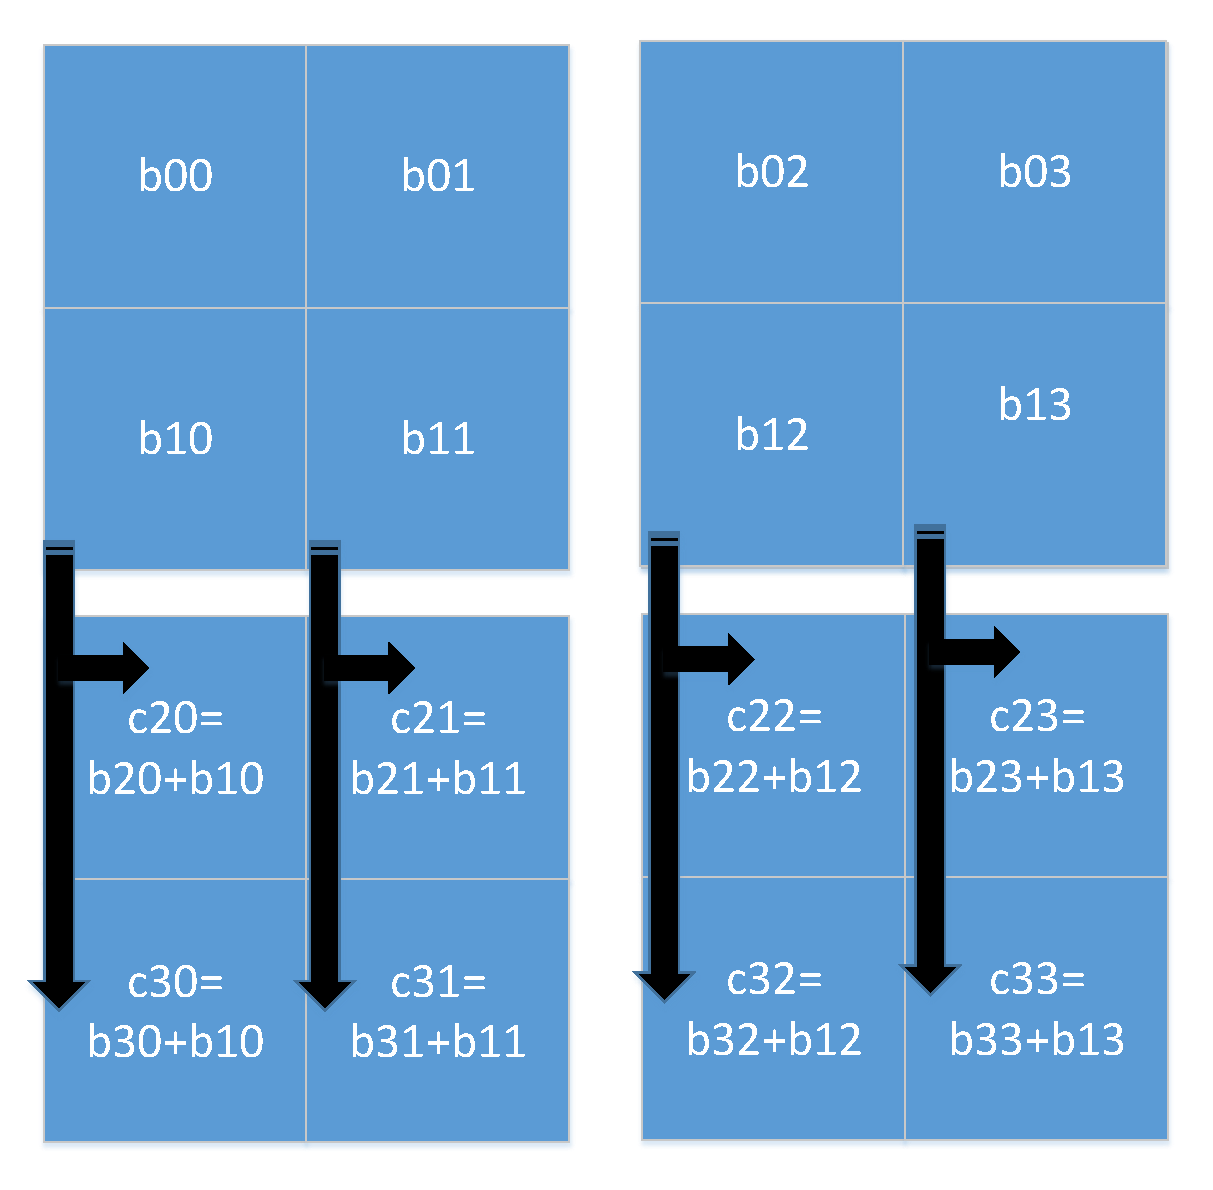
\includegraphics[scale=0.40]{imm/iia/iia_step2aa}  
   	   	\caption{Step 2-Sum vertically.}
   	   	\label{fig:IIA2aa}
   	   \end{figure}
   	   
   	   \begin{figure}[h]
   	   	\centering
   	   	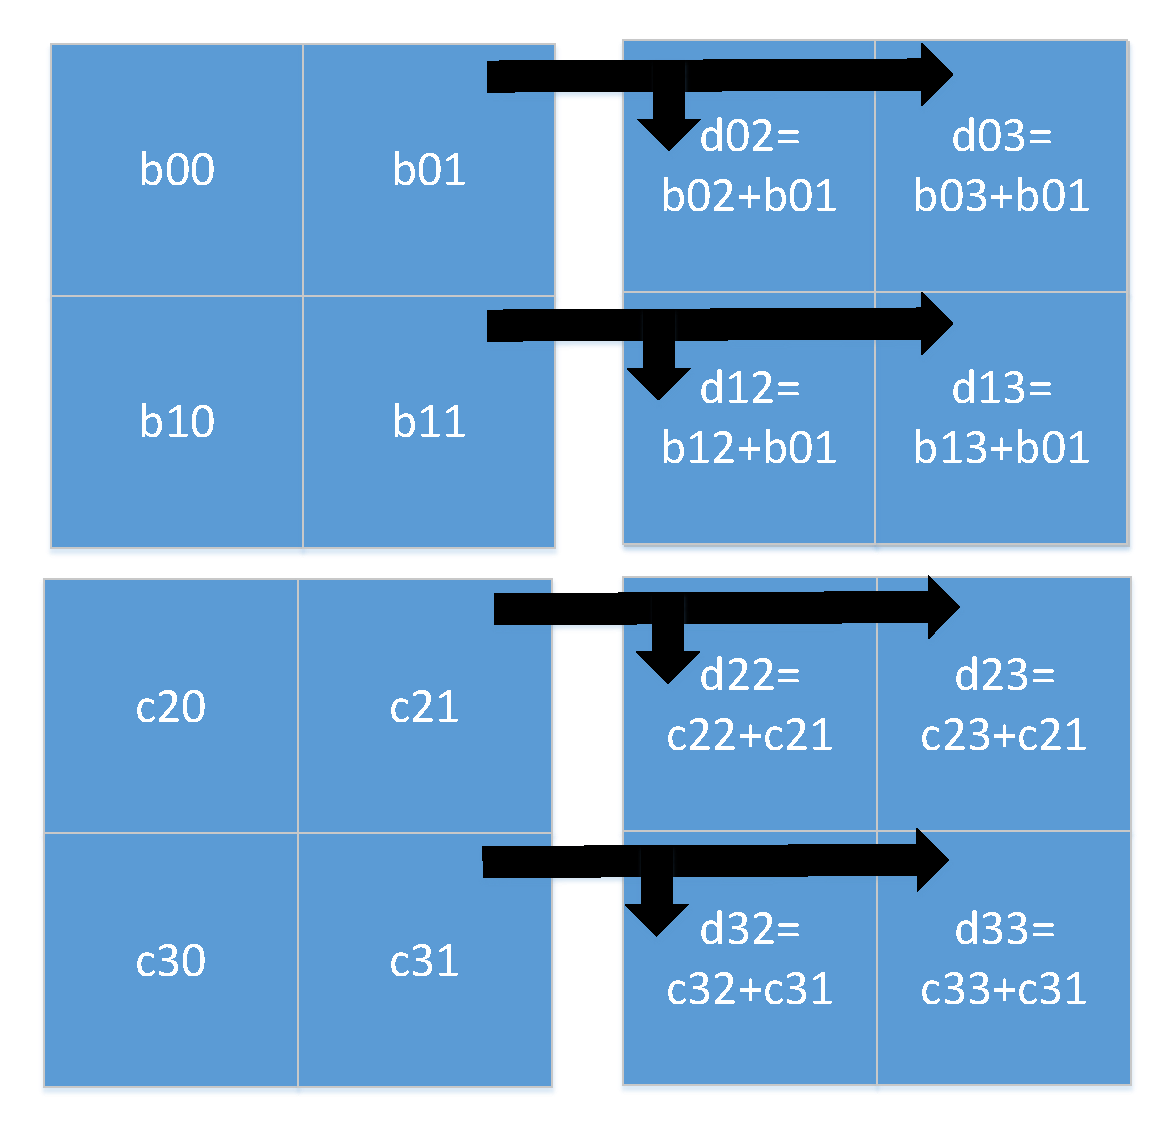
\includegraphics[scale=0.40]{imm/iia/iia_step2b}  
   	   	\caption{Step 2-Sum horizonatlly.} 
   	   	\label{fig:IIA2b}
   	   \end{figure}
  
   
   \item We repeat the prevoius step until we reach the matrix of dimension NxN
    \begin{figure}[h]
    	\centering	
    	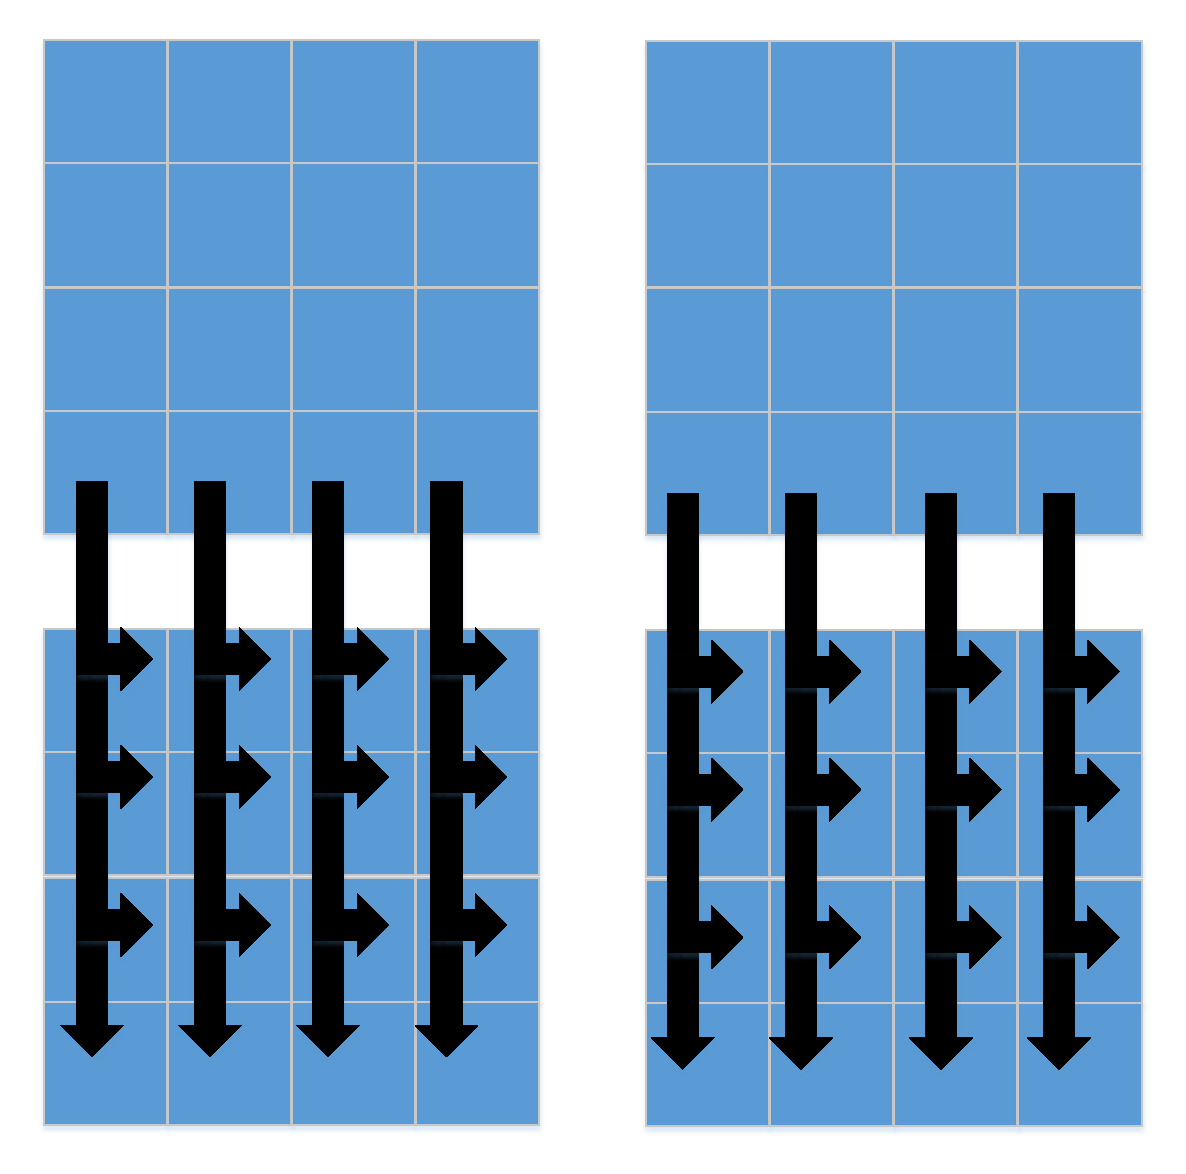
\includegraphics[scale=0.40]{imm/iia/iia_step3a}  
    	\caption{Step 3-Sum vertically.}
    	\label{fig:IIA3a}
    \end{figure}
    
    \begin{figure}[h]
    	\centering
    	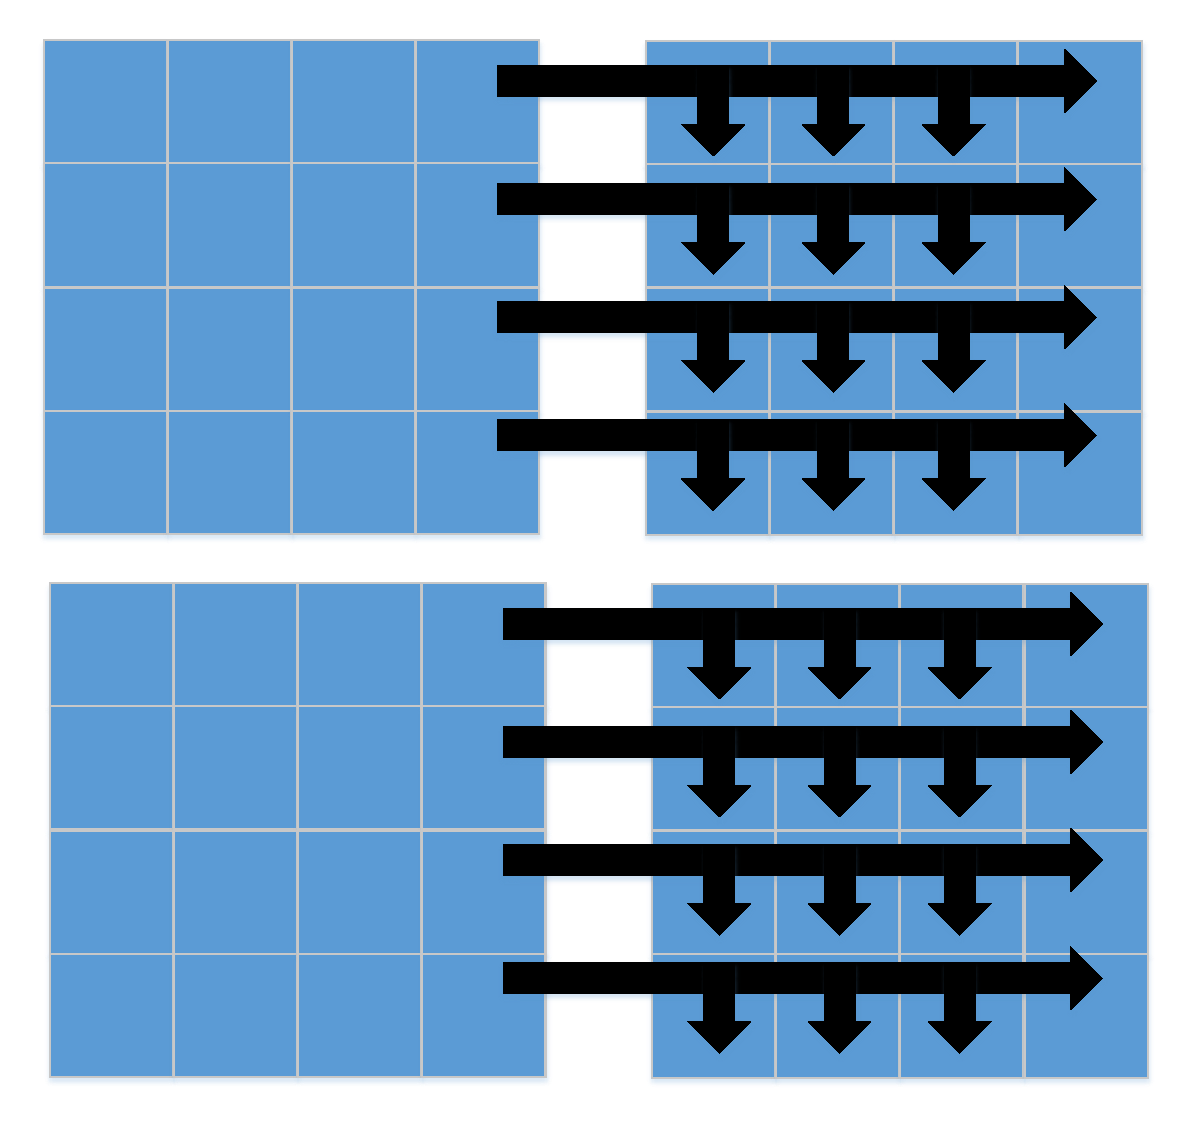
\includegraphics[scale=0.40]{imm/iia/iia_step3b}  
    	\caption{Step 3-Sum horizonatlly.} 
    	\label{fig:IIA3b}
    \end{figure}
     \end{enumerate}
     \clearpage
  \section{Pipelined Implementation}
  As explained before, in every step we divide the original matrix into small matrices of the size $ 2^i $x$ 2^i $ ( $ i $ represent the number of the actual step), and compute the SAT of each matrix independently from one another.
  The computed SATs will be used in the next step to evaluate the SATs of matrices with size $ 2^{i+1} $x$ 2^{i+1} $.
  We repeat this process until we reach the SAT of the original matrix. Figure \ref{fig:IIA_overall} represent the scheme of this implementation for a 8x8 matrix.
  The simbol $ \bigoplus $ means that it will evaluate the SAT of a matrix $ 2^{i+1} $x$ 2^{i+1} $ by using the SATs of 4 matrices $ 2^i $x$ 2^i $.
  By looking to the picture, we can clearly imagine to put some pipeline registers. This is possible because in each step $ i $ we need only the values calculated in the previous step $ i-1 $, we don't need the other values found in the other steps.
   
     \begin{figure}[h!]
     	\centering
     	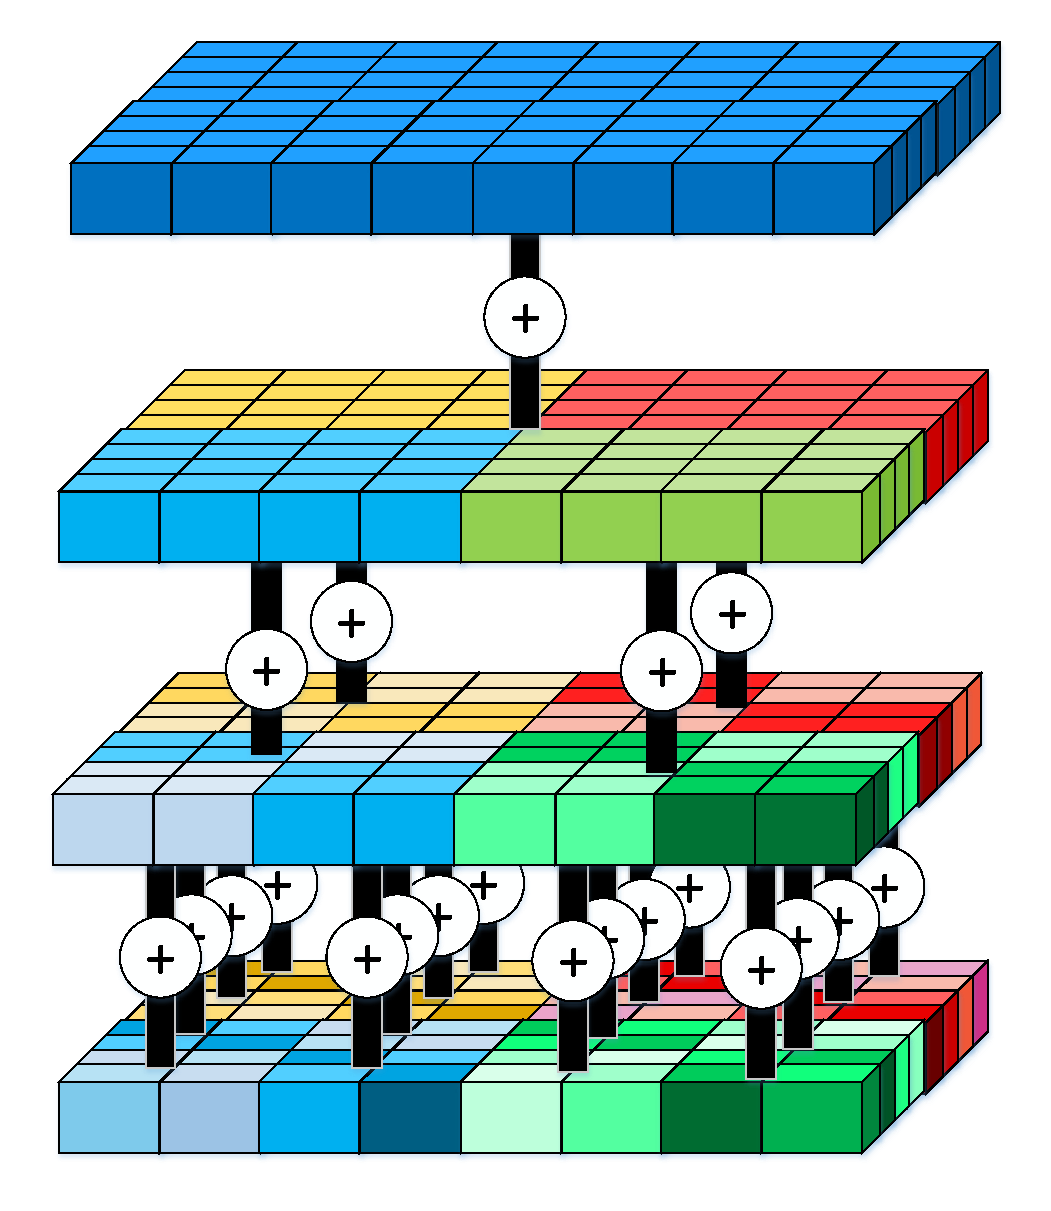
\includegraphics[scale=0.9]{imm/iia/iia_overall}  
     	\caption{Scheme of the SAT algorithm's imlementation.} 
     	\label{fig:IIA_overall}
     \end{figure}
     \clearpage
     \section{Simulation and Test}
     I did some tests of this implementation with different size and dimension. In the fig.\ref{fig:tb_iia} we can see the results of a matrix 4x4.
     
     \begin{figure}[h!]
     	\centering	
     	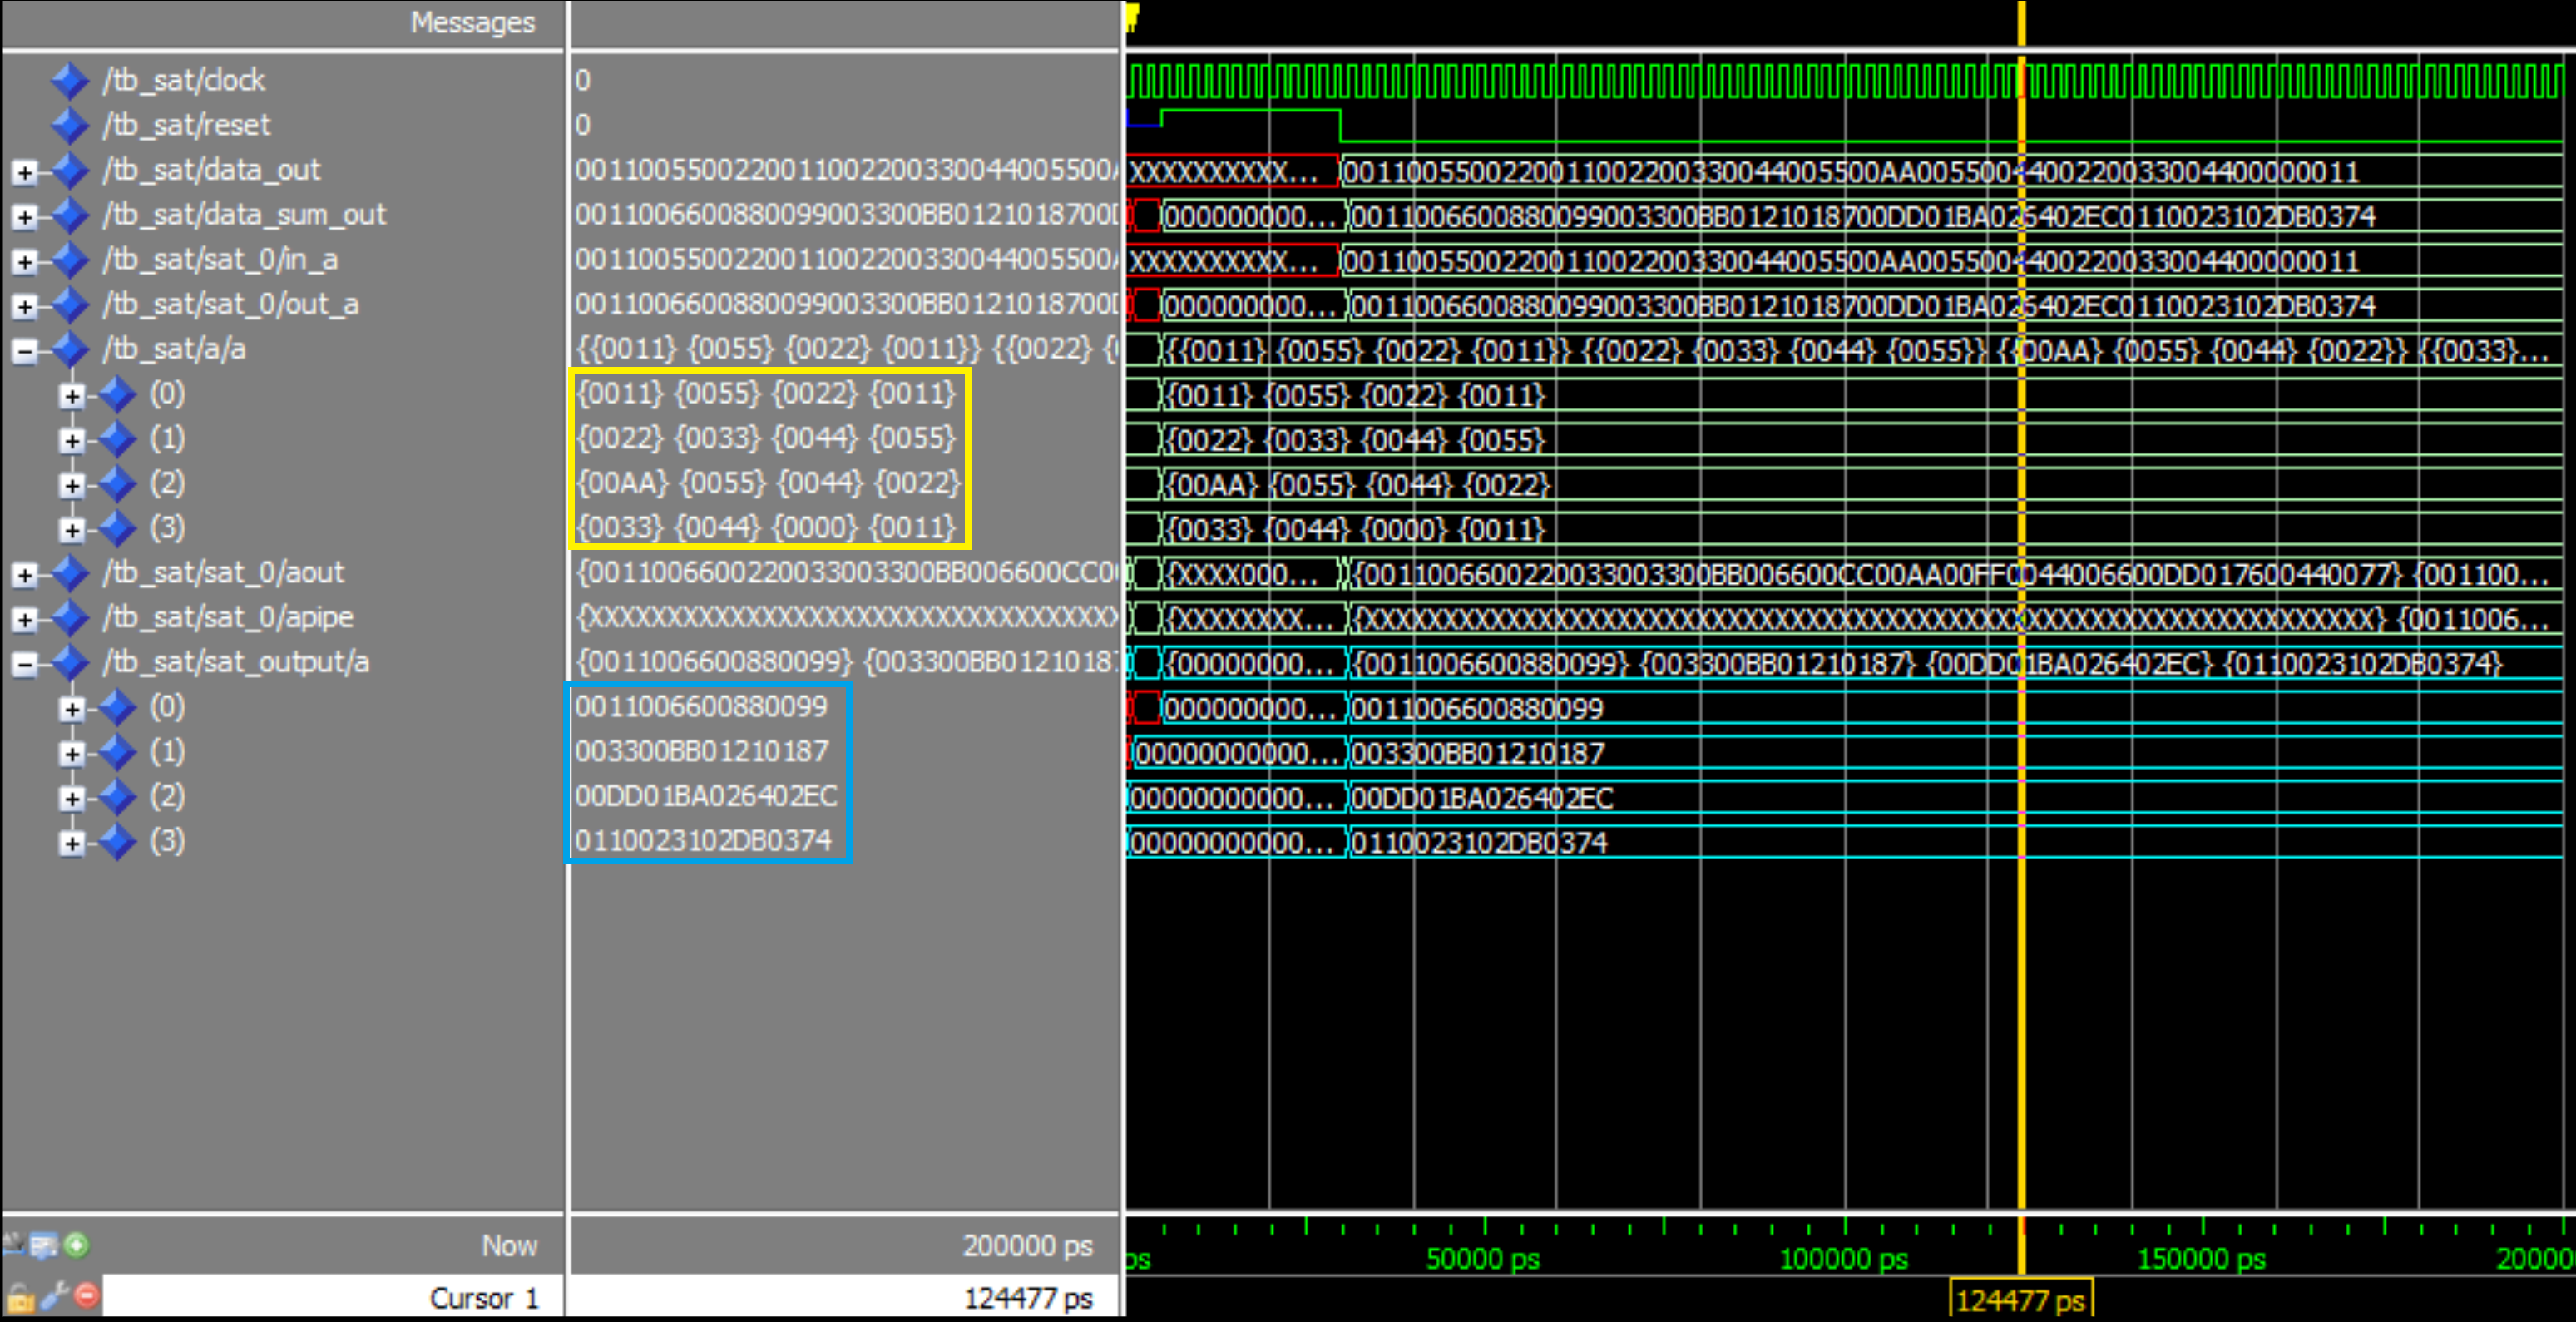
\includegraphics[width=\textwidth]{imm/iia/wave1.png}  
     	\caption{Integral Image-Results of the simulation} 
     	\label{fig:tb_iia}
     \end{figure}
     
     The input matrix is the one highlighted in yellow, while the output matrix is highlighted in light blue.
     We start from these values \begin{center}
     	$ 
     	\begin{bmatrix}
     	0x11 & 0x55 & 0x22 & 0x11\\
     	0x22 & 0x33 & 0x44 & 0x55   	\\
     	0xAA&0x55 & 0x44  &  0x22 \\
     	0x33& 0x44 & 0x0 & 0x11
     	\end{bmatrix}= 	\begin{bmatrix}
     	17 &   85 &   34 &   17\\
     	34  &  51  &  68  &  85\\
     	170  &  85  &  68  &  34\\
     	51    &68    & 0    &17\end{bmatrix}$
     \end{center}
     \bigskip
     we partition the original matrix in matrices 2x2
     \begin{center}
     	$ 
     	\begin{bmatrix}
     	\begin{pmatrix}
     	0x11 & 0x55\\
     	0x22 & 0x33
     	\end{pmatrix}&
     	\begin{pmatrix}
     	0x22 & 0x11\\
     	0x44 & 0x55 
     	\end{pmatrix}\\
     	&\\
     	\begin{pmatrix}
     	0xAA&0x55\\
     	0x33& 0x44
     	\end{pmatrix}&
     	\begin{pmatrix}
     	0x44  &  0x22\\
     	0x0 & 0x11
     	\end{pmatrix}
     	\end{bmatrix}
     =\begin{bmatrix}
     \begin{pmatrix}
     17 &85\\
      34& 51
     \end{pmatrix}&
     \begin{pmatrix}
     34 & 17\\
     68& 85 
     \end{pmatrix}\\
     &\\
     \begin{pmatrix}
     170&85\\
     51&68
     \end{pmatrix}&
     \begin{pmatrix}
     68  &34\\
     0 & 17
     \end{pmatrix}
     	\end{bmatrix}$
     \end{center}\bigskip
      and we perform the summed area table for each matrix 2x2
      \begin{center}
      	$ \begin{bmatrix}
      	\begin{pmatrix}
      	17 &17+85\\
      	34+17& 51+17+85+34
      	\end{pmatrix}&
      	\begin{pmatrix}
      	34 & 17+34\\
      	68+34& 85+17+34+68 
      	\end{pmatrix}\\
      	&\\
      	\begin{pmatrix}
      	170&85+170\\
      	51+170&68+170+85+51
      	\end{pmatrix}&
      	\begin{pmatrix}
      	68  &34+68\\
      	0+68 & 17+68+34
      	\end{pmatrix}
      	\end{bmatrix} =$
      \end{center}\bigskip
      \begin{center}
      	$\begin{bmatrix}
      	\begin{pmatrix}
      	17 &102\\
      	51& 187
      	\end{pmatrix}&
      	\begin{pmatrix}
      	34 & 51\\
      	102& 204 
      	\end{pmatrix}\\
      	&\\
      	\begin{pmatrix}
      	170&255\\
      	221&374
      	\end{pmatrix}&
      	\begin{pmatrix}
      	68  &102\\
      	68 & 119
      	\end{pmatrix}
      	\end{bmatrix}$
      \end{center}
      \bigskip
      If we translate it in hexdecimal we get
      \begin{center} \label{iia_matrix}
      	$ \begin{bmatrix}
      	\begin{pmatrix}
      	0x11 &0x66\\
      	0x33& 0xBB
      	\end{pmatrix}&
      	\begin{pmatrix}
      	0x22 & 0x33\\
      	0x66& 0xCC 
      	\end{pmatrix}\\
      	&\\
      	\begin{pmatrix}
      	0xAA&0xFF\\
      	0xDD&0x176
      	\end{pmatrix}&
      	\begin{pmatrix}
      	0x44  &0x66\\
      	0x44 &0x77
      	\end{pmatrix}
      	\end{bmatrix} $
      \end{center}
      \bigskip
      If we look the signal $ aout $ on the fig \ref{fig:tb_iia}, we can see the partial summed area table.
      \begin{center}
      	$ aout=0x0011006600220033003300BB006600CC00AA00FF0044006600DD017600440077 $
      \end{center}
      we know that each row has 4 elements of 16 bits
      \begin{center}
      	$ \begin{bmatrix}
      	1^{st}row=0x0011006600220033\\
      	2^{nd}row=0x003300BB006600CC\\
      	3^{rd}row=0x00AA00FF00440066\\
      	4^{th}row=0x00DD017600440077
      	\end{bmatrix} =\begin{bmatrix}
      	0x11 &0x66 & 0x22 & 0x33\\
      	0x33 & 0xBB &0x66&0xCC\\
      	0xAA&0xFF&0x44&0x66\\
      	0xDD&0x176&0x44&0x77
      	\end{bmatrix}$
      \end{center}
      which is the same we obtained above.\\
      Now we have to evaluate the summed area table of the matrix 4x4 by using the partial sum we have just found.
      As described before (section \ref{hiiia}), when we sum vertically, we sum to all the lower half cells with the corresponding cell of the last row of the upper half matrix. Similarly we sum horizontally
      \begin{center}
      	$  \begin{matrix}
      	
      	\begin{bmatrix}
      	17 &102 & 34 & 51\\
      	51 &187 &102&204\\
      	170&255&68&102\\
      	221&374&68&119
      	\end{bmatrix}\\
      	\Downarrow\\
       	\end{matrix}$\\
       	sum vertically\\
       	$ \Downarrow $\\
       	$\begin{matrix}
       	
      	\begin{bmatrix}
      	17 &102 & 34 & 51\\
      	51 &187 &102&204\\
      	170+51&255+187&68+102&102+204\\
      	221+51&374+187&68+102&119+204
      	\end{bmatrix}
      	\\\Downarrow
      	\end{matrix}$\\
      	sum horizontally\\
      	$ \Downarrow $\\$
      	\begin{bmatrix}
      	17 &102 & 34+102 & 51+102\\
      	51 &187 &102+187&204+187\\
      	221&442&170+442&306+442\\
      	272&561&170+561&323+561
      	\end{bmatrix}$
      \end{center}
      \bigskip
      Finally we get        
     \begin{center}
     	$ \begin{bmatrix}
     	17&   102&   136&   153\\
     	51 &  187 &  289 &  391\\
     	221  & 442  & 612  & 748\\
     	272   &561   &731   &884\\
     	\end{bmatrix}=
     	\begin{bmatrix}
     	0x11 & 0x66 & 0x88 & 0x99\\
     	0x33 & 0xBB & 0x121 & 0x187   	\\
     	0xDD&0x1BA & 0x264  &  0x2EC \\
     	0x110& 0x231 & 0x2DB & 0x374
     	\end{bmatrix}$
     \end{center}
     Which is the same result given in the simulation (fig \ref{fig:tb_iia}, signal $ sat\_output/a $) and also by MATLAB as shown below
      \begin{figure}[h!]
      	\centering	
      	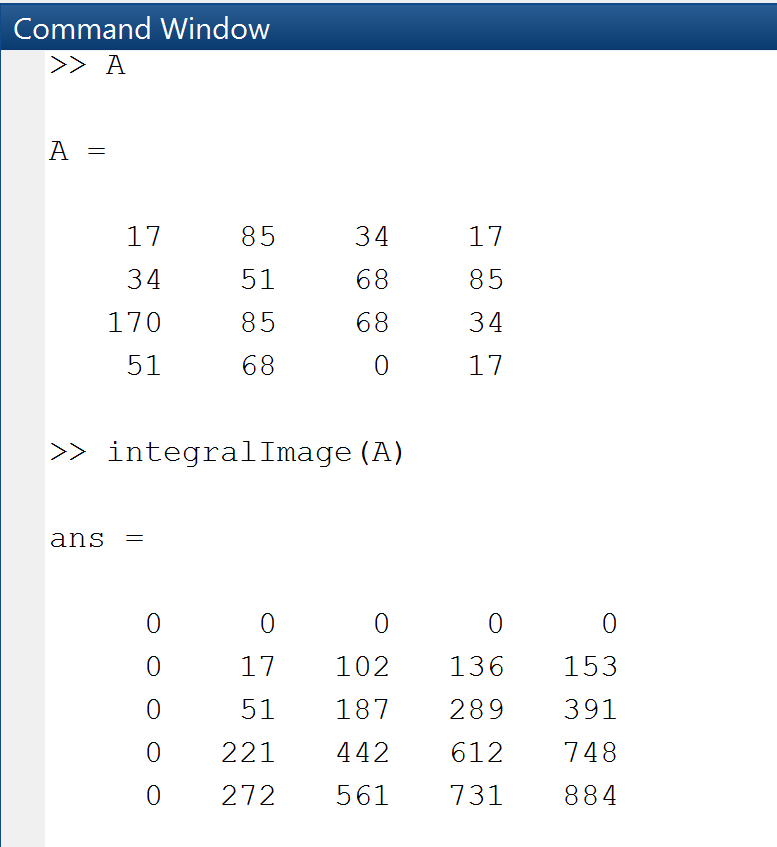
\includegraphics[width=0.8\textwidth]{imm/iia/iia_mat.png}  
      	\caption{Integral Image-Checking with MATLAB} 
      	\label{fig:iia_mat}
      \end{figure}
 \clearpage
 \section{Comparison}
 There are two typical existed image integral algorithms on GPUs. The first is the Inclusive Scan algorithm. The second is the Balanced Trees Parallel Scan algorithm. Compared with the Inclusive Scan algorithm, the proposed scheme reduces logarithmically the global computation time without any pipeline (with pipeline, the improvement will be even greater). Compared with the Balanced Trees Parallel Scan algorithm, the proposed algorithm only needs about half of the global computation time.
 The theoretical implementation shows that the proposed algorithm gets the best performance compared with the two above integral algorithms.
 
 
 \subsection{Inclusive Scan algorithm}
 We perform the inclusive scan for each row and evaluate the partial sum.
 Finally we perform the inclusive scan for each column.
 Figure \ref{fig:inclusive_scan} shows an example of this implementation for a matrix 3x3. \cite{sat3}
 
   \begin{figure}[h!]
   	\centering
   	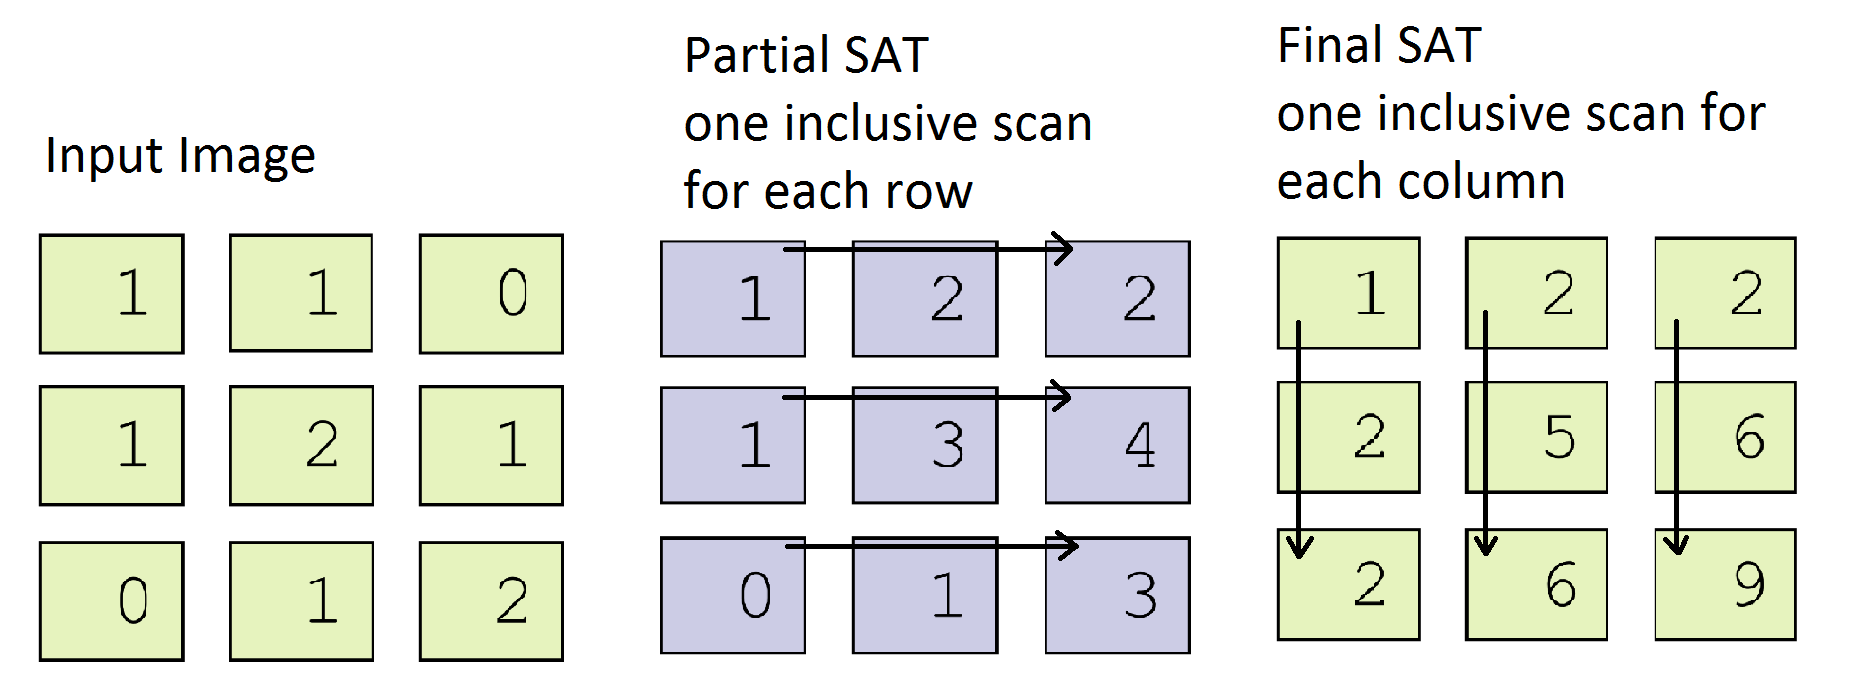
\includegraphics[width=\textwidth]{imm/iia/inclusive_scan}  
   	\caption{Scheme of the inclusive scan algorithm} 
   	\label{fig:inclusive_scan}
   \end{figure}
 
 \subsection{Balanced Trees Parallel Scan algorithm}
 For simplicity, i will explain the algorithm for a 1D-array.
 The goal is to evaluate the SAT of a single row which is also known as the prefix sum, also called cumulative sum, inclusive scan. \cite{sat1}
 
 A prefix sum can be calculated in parallel by the following steps.

 \begin{enumerate}
 \item Build a balanced binary tree on the input data and sweep it to and from the root. 
 \item Traverse down from leaves to root building partial sums at internal nodes in the tree. 
 \item Traverse back up the tree building the scan from the partial sums.
 \end{enumerate}
 
  
 Figure \ref{fig:Balanced_tree} shows the scheme for an array of dimension 16.
 For a matrix, we implement this algorithm for each row and then for each column.
 
 \begin{figure}[h!]
 	\centering
 	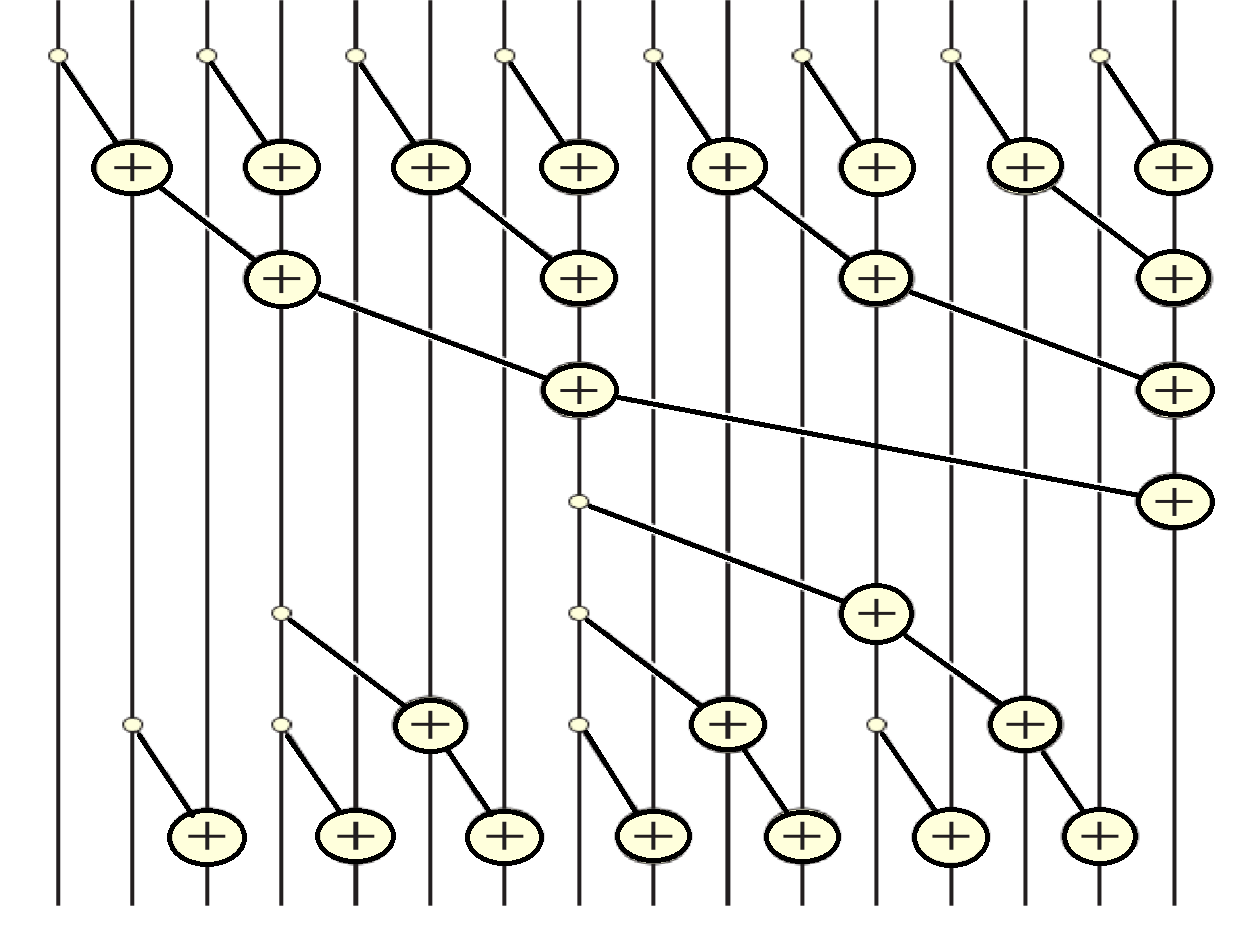
\includegraphics[width=\textwidth]{imm/iia/Balanced_tree0}  
 	\caption{Parallel Balnced Tree Algorithm for a 1D array} 
 	\label{fig:Balanced_tree}
 \end{figure}
 
\subsection{Comparing the 3 algorithm implementations}
Now that we know the implementation of these algorithm we can compare the area, i.e. the number of adders required, and the time between them.
In the table \ref{table:iia_tab} the unit time $ t $ is the time required to get the result of a single sum.


\begin{center}
	\begin{tabular}{ | p{1.7cm} | c | c | c | c |}
			
		\hline
		\label{table:iia_tab} & Inclusive scan & Balanced tree & This work & This work pipelined\\
		\hline
		Area & $ 2N(N-1) $ & $ 2N(2N-log_2 N -2) $ & $ N\cdotp N\cdotp log_2 N$ & $ N\cdotp N $\\
		\hline
		Time & $ 2(N-1) \cdotp t $
		& $ 2(2
		log_2 N-1)t $ &
		$ (log_2 N)2t $ & $ 2t $ \\
		\hline
		
	\end{tabular}
\end{center}
\subsection{Logic-In-Memory architecture} \label{sssec:1}
The \textit{Logic-In-Memory} is  a new architecture where logic and memory are embedded as unique entity instead of two separated ones (fig. \ref{fig:A}). \cite{lim}

The memory is made of small entities called \textit{bricks} populating two different layers: the bricks of each layer can communicate each other like in a matrix structure and only specifc bricks, called \textit{pillars}, are allowed to exchange data with the upper layer(fig. \ref{fig:B}). 
\begin{figure}[h!]
	\centering
	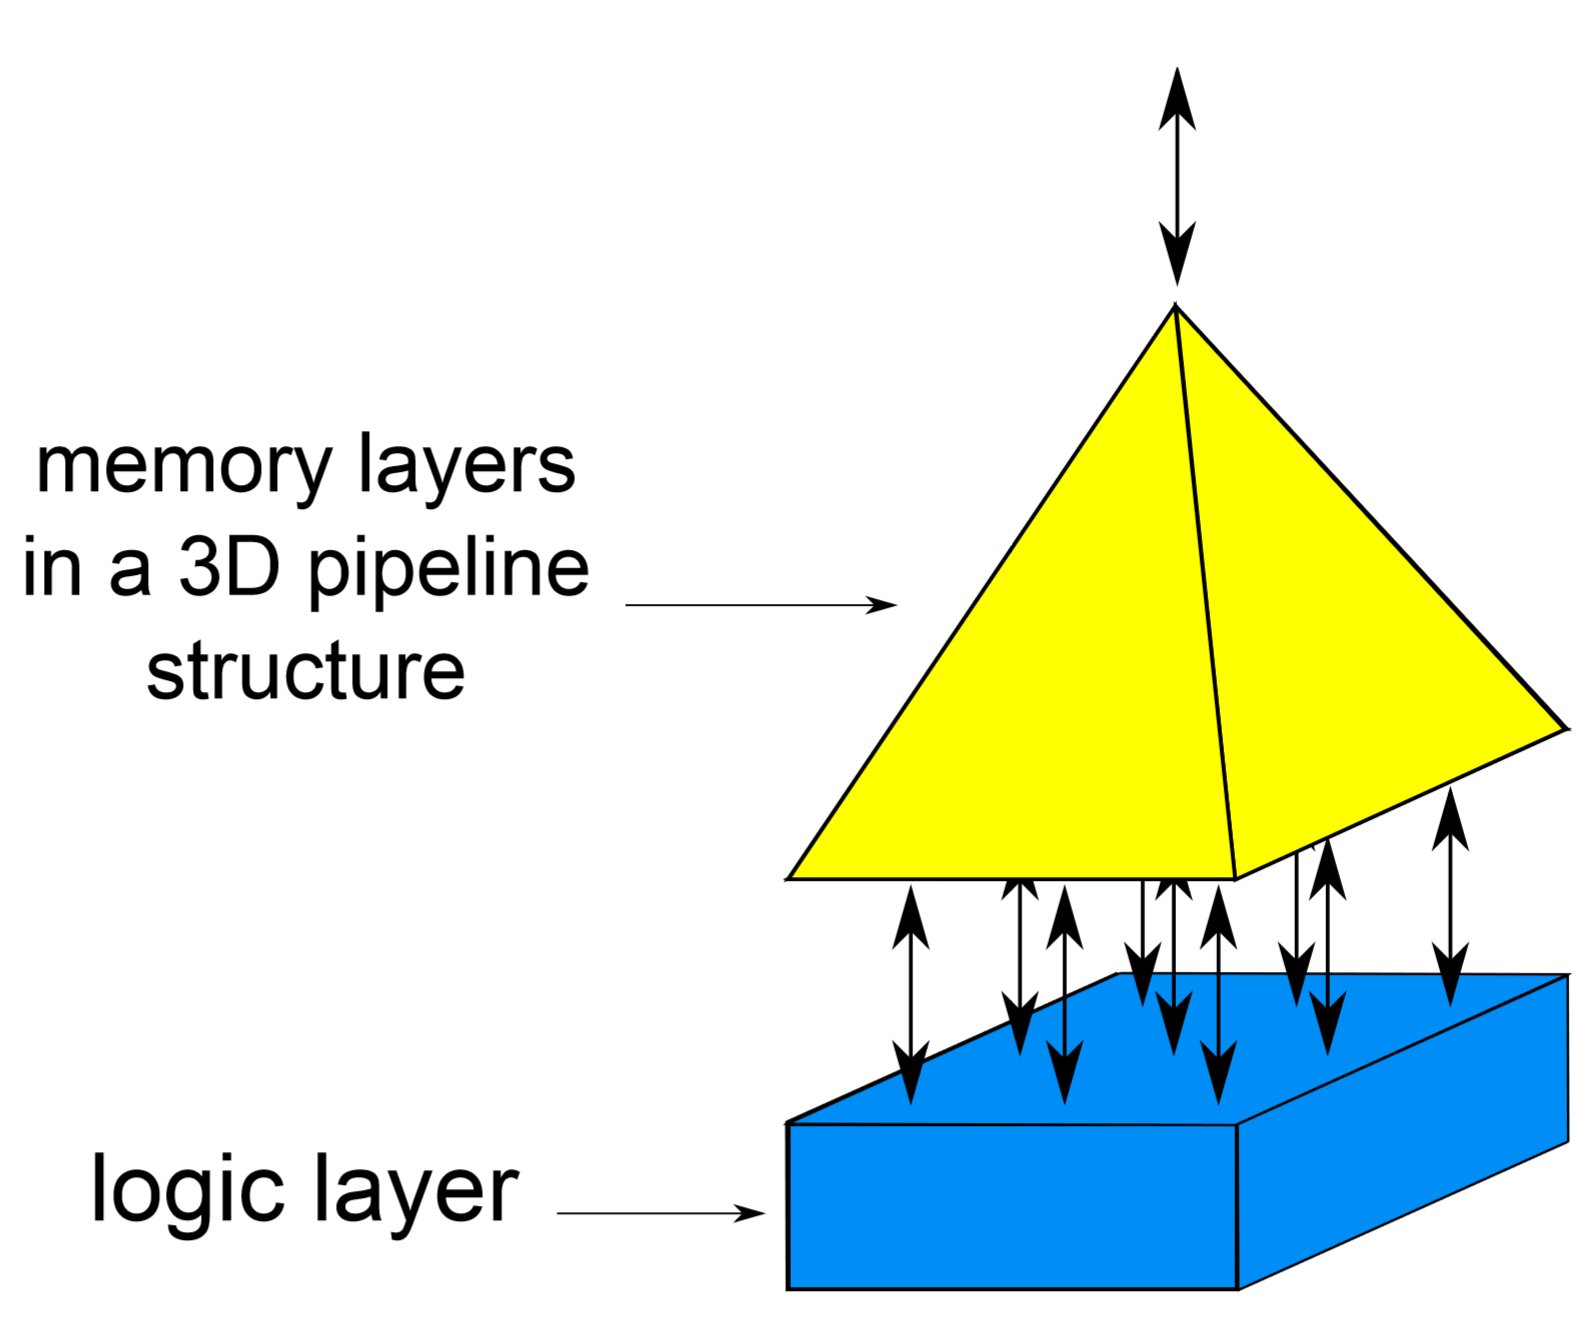
\includegraphics[width=\textwidth]{imm/iia/A.png}  
	\caption{Graphics representation of the architecture 2.0: the yellow pyramid represent the 3D pipeline of smart memories whereas the blue layer represent the programmable logic layer.} 
	\label{fig:A}
\end{figure}

\begin{figure}[h!]
	\centering
	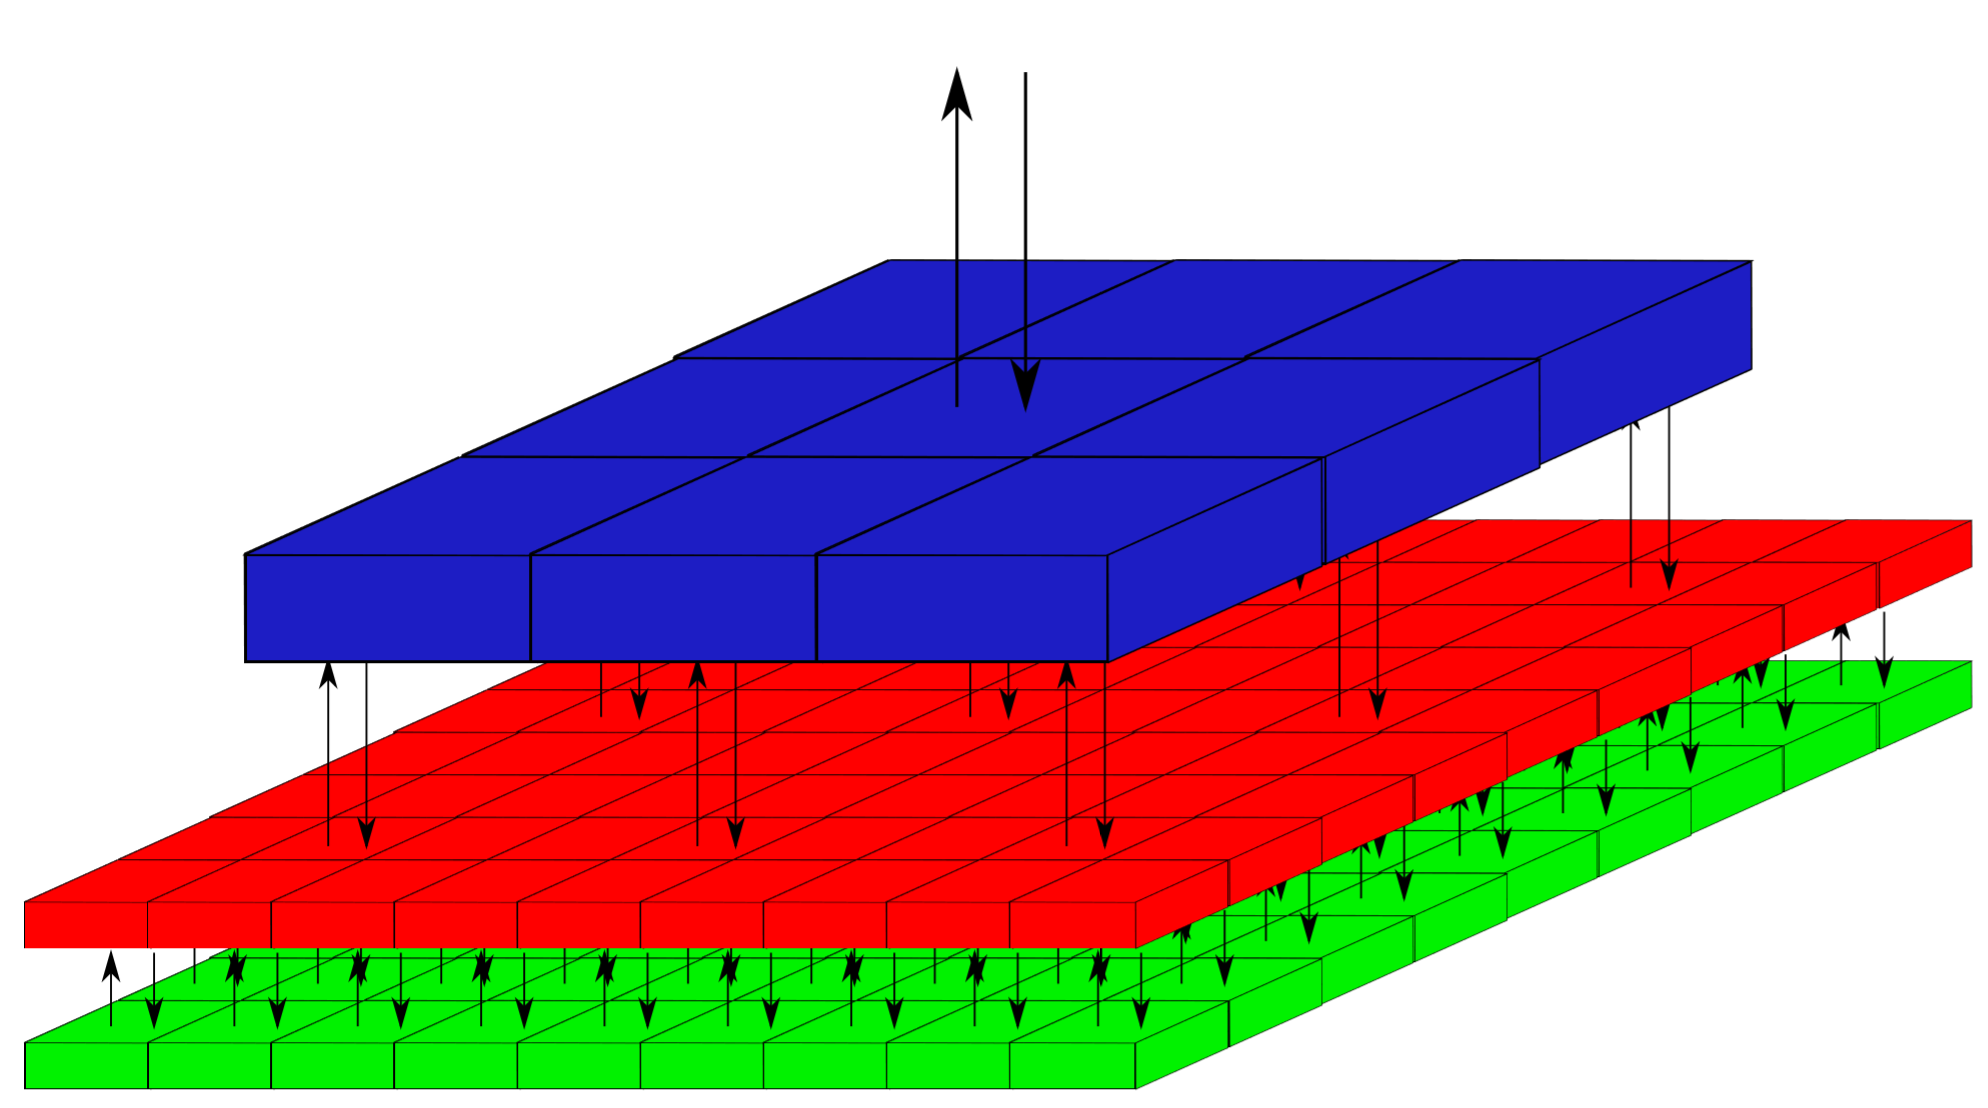
\includegraphics[width=\textwidth]{imm/iia/B.png}  
	\caption{ Structure of the LIM. The green layer represent the logic and is composed of 81 ALUs communicating each one with every brick of the bottom layer (red); the blue layer represent the upper plane and is composed of 9 bricks, one every 9 bricks of the bottom layer. Only the pillars of the bottom layer can communicate with the upper layer; only the pillar of the upper layer can exchange data with the outside.
	} 
	\label{fig:B}
\end{figure}
The upper layer is composed of a smaller number of bricks having a bigger memory capacity than the ones in the bottom layer: here the bricks are more in number but their memory capacitance is small. In addition, only this plane is able to communicate with the programmable logic layer: it is made of one ALU (arithmetic and logic unit) for each brick of the bottom layer. 
\clearpage
\subsection{Comparison with the LIM architecture}
I take the results of the LIM's architecture
 The pseudocode for the LIM architecture is the following:
 \begin{enumerate}
 	\item Each cell reads its own value;
 	\item Sums its value to the one received from the NORTH and sends the result to the SOUTH;
 	\item Samples the value coming from the WEST, sums it to the previous result and sends it to the EAST;
 	\item Writes the final result in its own memory;
\end{enumerate}
 The main advantage of the LIM architecture is the parallelism: the presence of many cells that can work autonomously greatly increases the speed of the computation of algorithms that can be executed in parallel.
  The duration of the algorithm depends on the number of cells of the grid: in particular, supposing to have a grid of $ N \cdot N  $ cells, the total duration is equal to:
  \begin{itemize}
  	\item N clock cycles to write the data; 
  	\item 6N clock cycles to compute the algorithm; 
  	\item 2N+1 clock cycles to read the data through a remote read.   	
  \end{itemize} 
  Therefore,
  \begin{center}
  	$ t = N +6N +2N +1=9N +1 $
  \end{center}
  
  	 \begin{center}
  	 	\begin{tabular}{ | p{1.7cm} | c | c | c |}
  	 		
  	 		\hline
  	 		\label{table:iia2_tab} & LIM & This work & This work pipelined\\
  	 		\hline
  	 		Area & $ N\cdotp N$ cells  &  $ N\cdotp N\cdotp log_2 N $ adders  & $ N\cdotp N $ adders\\
  	 		\hline
  	 		Time & $ 9N +1  $ cycles
  	 		&
  	 		Time for $ 2(log_2 N) $ adders &Time for $ 2 $ adders\\
  	 		
  	 		\hline
  	 		
  	 	\end{tabular}
  	 \end{center}
\section{Characteristics of the Integral Image Algorithm}
\vspace{10pt}
{\large \textbf{PROCESSING ELEMENTS}}\vspace{10pt}\\
\begin{tabular}{ p{0.2cm} p{14.5cm}}
	
&\textbf{1- Which kind of Processing element?}\\
&	Adder\vspace{7pt}\\
&	\textbf{2- Functionality}\\
&	Addition, summation\vspace{7pt}\\
&	\textbf{3- Complexity}\\
&	\begin{tabular}{ p{0.2cm} p{3cm} p{7cm}}
		
		&Not pipelined & Area $ N\cdot N\cdot log_2(N) $ adders\\
		& & Time$ (log_2N)2 $x(time for an addition) \vspace{3pt}\\
		& Pipelined & Area $ N^2 $ adders\\
		& & Time $ 2 $x(time for an addition)\\
		
	\end{tabular}\vspace{7pt}\\
&	\textbf{4- Parallelism}\\
&	All cells perform their Integral Image value in parallel.\vspace{7pt}\\
&	\textbf{5-Reconfigurability}\\
&	No\vspace{7pt}\\
&	\textbf{6- Programmability}\\
&	No\vspace{7pt}\\
&	\textbf{7- Need a dedicated memory?}\\
&	If the architecture is pipelined, you need to store the partial sum.\\
&	If not pipelined, no memory is required.\vspace{7pt}\\
	&\textbf{8- Relationship with I/O}\\
&	INPUT: values of the matrix's cells\\
&	OUTPUT: result of the integral image algorithm\end{tabular}\vspace{24pt}\\
\clearpage
{\large \textbf{\qquad }}\vspace{10pt}\\
{\large \textbf{MEMORY ELEMENTS}}\vspace{10pt}\\\begin{tabular}{ p{0.2cm} p{14.5cm}}
&\textbf{1- Need a clever memory LIM?}\\
&	No, but can be implemented\vspace{7pt}\\
&\textbf{2- Is there a data search algorithm?}\\
&	No\vspace{7pt}\\
&\textbf{	3-Interface mechanism with other PE or memories}\\
&	Communication required between cells (even between distant cells e.g. the center cell and the last cell).\vspace{7pt}\\
&	\textbf{4- Access mechanism}\\
&	(No memory for this implementation)\vspace{7pt}\\
&	\textbf{5- Hierarchization} \\
&	(No memory for this implementation)\vspace{7pt}\\
&\textbf{	6- Cache coherency} \\
&	(No memory for this implementation)\vspace{7pt}\\
&\textbf{	7- Is it a a transactional memory?}\\
&	(No memory for this implementation)\vspace{7pt}\\
&\textbf{	8- Are there virtualization (paging) mechanisms?}\\
&	(No memory for this implementation)\end{tabular}\vspace{14pt}\\
\vspace{10pt}\\
{\large\textbf{ENCODING INFORMATION}}\vspace{10pt}\\
\begin{tabular}{ p{0.2cm} p{14.5cm}}
	&\textbf{1-Which encoding is used?}\\
	&Binary encoding
\end{tabular}
\newpage
{\large\textbf{ }}\vspace{10pt}\\
{\large\textbf{CONNECTIONS}}\vspace{10pt}\\\begin{tabular}{ p{0.2cm} p{14.5cm}}
&\textbf{1-Packet Exchange Protocol}\\
&Directly\vspace{7pt}\\
&\textbf{2-Timing (asynchronou/synchronous)}\\
&Synchronous\vspace{7pt}\\
&\textbf{3-Are there multiple instances? }\\
&Yes, but the summation is not the same for all (some cells requires more data exchanging than others)\vspace{7pt}\\
&\textbf{4-Heterogeneity (Local/Distant I/O Connections)}\\
&Heterogeneous when storing the initial values to the cells, not heterogeneous when exchanging the data (sometimes you exchange data between local cells, the other times you exchange between distant cells.)\vspace{7pt}\\
&\textbf{5-Are there any buffers?}\\
&There are pipeline registers.
\end{tabular}\vspace{14pt}\\
